\documentclass[12pt]{article}
\usepackage[utf8]{inputenc}
\usepackage{amsmath,amsfonts}
\usepackage{hyperref}
\usepackage{tikz}
\usepackage{pgfplots}
\usepackage{xcolor}
\definecolor{myblue}{rgb}{0.00,0.39,0.67}
\definecolor{myred}{rgb}{0.86,0.08,0.14}
\definecolor{mygreen}{rgb}{0.07,0.52,0.07}
\definecolor{myorange}{rgb}{0.99,0.32,0.08}
\definecolor{mygray}{rgb}{0.5,0.5,0.5}
\def\happy{\mathcal{H}}
\def\gym{\mathcal{G}}
\def\bonus{\mathcal{B}}
\def\Sc{S_\text{cap}}
\def\Ec{E_\text{cap}}

\begin{document}
\begin{center}
    \bf\Huge Battle stats formula
\end{center}

\section{Gym gain formula}
From \href{https://www.torn.com/forums.php?p=threads&f=61&t=16003284&b=0&a=0&start=0&to=17684755}{Vladar [1996140]}.
This formule gives the stat gains as a function of the current stat, the energy spent on train and a other parameters.

\par In this formula and for the rest we will need:
\begin{itemize}
    \item 2 variables and there increment
    \begin{itemize}
        \item Energy $E$ and $dE$
        \item Stat $S$ and $dS$
    \end{itemize}
    \item 6 known coefficients
        \begin{itemize}
            \item $a = 0.0000003480061091$
            \item $b = 250$
            \item $c = 0.000003091619094$
            \item $d = 0.0000682775184551527$
            \item $e = -0.0301431777$
            \item $\Sc = 50000000$ (known as the stat cap)
        \end{itemize}
    \item 3 states variables
    \begin{itemize}
        \item Happy level $\happy$
        \item Gym coefficient $\gym$
        \item Gym gain bonus $\bonus$
    \end{itemize}
\end{itemize}

The Valdar formula eq.\eqref{eq:valdar} gives the stat gains $dS$ as a function of the current stat $S$ and the energy spent $dE$. It is usually written:
\begin{equation}
    dS = \left[ (a\ln(\happy+b)+c) \bar{S} + d(\happy+b) + e \right](1+\bonus)\gym dE
    \label{eq:valdar}
\end{equation}
with $\bar{S} = \min(\Sc, S)$

\par By introducing 2 new parameters $\alpha$ and $\beta$ that depends only on the 5 coefficients $a, b, c, d, e$ and the state variables $\happy, \bonus, \gym$, eq.\eqref{eq:valdar} can be written as follow:
\begin{equation}
    \frac{dS}{dE} = \alpha \bar{S} + \beta \quad \Leftrightarrow \quad \frac{dS}{dE} - \alpha \bar{S} = \beta
    \label{eq:valdar-diff}
\end{equation}
with
\begin{equation}
    \left\{\begin{aligned}
        \alpha &= (a\ln(\happy+b)+c)(1+\bonus)\gym\\
        \beta &= (d(\happy+b) +e)(1+\bonus)\gym
    \end{aligned}\right.
\end{equation}

\section{Battle stats formula: $S(E)$}
\par {\color{myred}\bf Assumption: $\happy$, $\gym$ and $\bonus$ remain constant (which is not realistic for a long term prediction at early stages).}

\par From eq.\eqref{eq:valdar-diff} it can clearly be seen that the $S(E)$ is driven by a simple ODE. Because of the piece wise definition of the equation the two cases $S<\Sc$ (before cap) and $S>\Sc$ (after cap) have to be treated separatly.

\subsection{Before cap}
With $S<\Sc$ eq.\eqref{eq:valdar-diff} can be written:
\begin{equation}
    \frac{dS}{dE} -\alpha S = \beta
\end{equation}
Which leads to the solution:
\begin{equation}
    \forall k \in \mathbb{R},\quad S(E) = ke^{\alpha E} - \frac{\beta}{\alpha}
\end{equation}
With the initial condition $S(0)=0$ we have
\begin{equation}
    S(E) = \frac{\beta}{\alpha}\left(e^{\alpha E} - 1\right)
    \label{eq:bs-bc-diff}
\end{equation}

It can be interesting to compute $E=\Ec$ such that $S(\Ec)=\Sc$ which can be done by inverting eq.\eqref{eq:bs-bc-diff}. It gives:
\begin{equation}
    \Ec = \frac{1}{\alpha}\ln\left(\frac{\alpha \Sc}{\beta} +1 \right)
\end{equation}

\subsection{After cap}
With $S<\Sc$ eq.\eqref{eq:valdar-diff} can be written:
\begin{equation}
    \frac{dS}{dE}  = \alpha \Sc + \beta
\end{equation}
which directly yields
\begin{equation}
    \forall k \in \mathbb{R},\quad S(E)  = (\alpha \Sc + \beta) E + k
\end{equation}
With the condition $S(\Ec)=\Sc$ we have:
\begin{equation}
    \begin{aligned}
        S & = (\alpha \Sc + \beta)E + \Sc - (\alpha \Sc + \beta) \Ec \\
          & = (\alpha \Sc + \beta) (E - \Ec) + \Sc
    \end{aligned}
\end{equation}

\begin{figure}[!h]
    \centering
    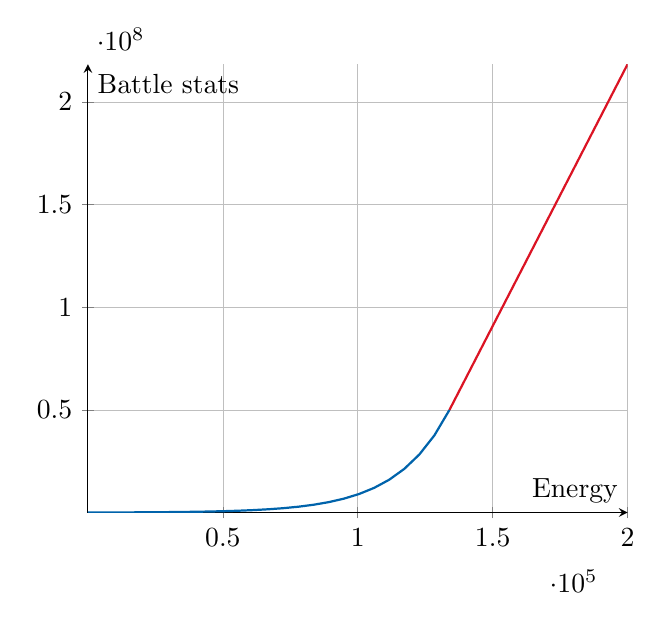
\begin{tikzpicture}
        \begin{axis}[
            % xmin=0,xmax=5000000,
            % ymin=0,ymax=100000000,
            grid=both,
            grid style={line width=.1pt, draw=gray!10},
            major grid style={line width=.2pt,draw=gray!50},
            axis lines=middle,
            % minor tick num=4,
            % ticks=none,
            ylabel=Battle stats,
            xlabel=Energy
        ]

           % \def\alpha{0.0000052543};
           % \def\beta{0.0039955815};
           % \def\ec{2111332.2434403603};
           % \def\sc{50000000)};
           % \addplot[myblue, domain=0:\ec, thick]{ \beta * (exp(\alpha * x) - 1) / \alpha };
           % \addplot[myred, domain=\ec:2500000, thick]{ (\alpha * \sc + \beta) * (x - \ec) + \sc };
           \def\alpha{0.0000509798};
           \def\beta{2.7561943022};
           \def\ec{133988.1087149439};
           \def\sc{50000000)};
           \addplot[myblue, domain=0:\ec, thick]{ \beta * (exp(\alpha * x) - 1) / \alpha };
           \addplot[myred, domain=\ec:200000, thick]{ (\alpha * \sc + \beta) * (x - \ec) + \sc };
           % \addplot[myred,  domain=0:40, thick]{ 100 };
           % \draw   [mygreen, thick] (axis cs:0,95) -- (axis cs:21.65,95) -- (axis cs:21.65,0);

           \end{axis}
    \end{tikzpicture}

    \caption{Battle stats as a function of energy for $\happy = 5000$, $\gym = 7.3$ and $\bonus= 15\%$}
\end{figure}



\end{document}
